\documentclass{beamer}
\usepackage{subcaption}
\usepackage{natbib}
\usepackage{tikz}
\usepackage{tikz-qtree}
\usepackage{mathtools}
%\usepackage{pifont}
\newcommand{\smallspace}{\hspace{1mm}}

\mode<presentation> {
\usetheme{Madrid}

% \usecolortheme{albatross}
% \usecolortheme{beaver}
% \usecolortheme{beetle}
% \usecolortheme{crane}
% \usecolortheme{dolphin}
% \usecolortheme{dove}
% \usecolortheme{fly}
% \usecolortheme{lily}
% \usecolortheme{orchid}
% \usecolortheme{rose}
% \usecolortheme{seagull}
% \usecolortheme{seahorse}
% \usecolortheme{whale}
% \usecolortheme{wolverine}

% \setbeamertemplate{footline} % To remove the footer line in all slides uncomment this line
% \setbeamertemplate{footline}[page number] % To replace the footer line in all slides with a simple slide count uncomment this line

\setbeamertemplate{navigation symbols}{} % To remove the navigation symbols from the bottom of all slides uncomment this line
}

%\usepackage{graphicx} % Allows including images
\usepackage{booktabs} % Allows the use of \toprule, \midrule and \bottomrule in tables

%%----------------------------------------------------------------------------------------
%%	TITLE PAGE
%%----------------------------------------------------------------------------------------

\title[RL of Theorem Proving]{Reinforcement Learning of Theorem Proving} % The short title appears at the bottom of every slide, the full title is only on the title page

%\author{Dobrik Georgiev} % Your name
%\institute[Cambridge] % Your institution as it will appear on the bottom of every slide, may be shorthand to save space
%{
%\textit{dgg30@cam.ac.uk.com} % Your email address
%}
%\date{} % Date, can be changed to a custom date

\begin{document}

\begin{frame}
\titlepage % Print the title page as the first slide
\end{frame}

\begin{frame}
\frametitle{Overview} % Table of contents slide, comment this block out to remove it
\tableofcontents % Throughout your presentation, if you choose to use \section{} and \subsection{} commands, these will automatically be printed on this slide as an overview of your presentation
\end{frame}
\section{Connection Tableau} 

\begin{frame}
    \frametitle{Connection Tableau}
    \begin{columns}
        \column{.45\textwidth}
        \begin{align*}
            &\begin{aligned}
                \{P,\smallspace R\} \smallspace
                \{\neg{P},\smallspace f(X) \}\smallspace
                \{\neg{f(b) },\smallspace P\}\smallspace
            \end{aligned}\\
            &\begin{aligned}
                \{\neg{f(c) },\smallspace \neg{P}\}\smallspace
                \{P,\smallspace \neg{P}\}
            \end{aligned}
        \end{align*}
        \column{.45\textwidth}
                \centering
                \only<1>{
                    \begin{tikzpicture}
                    \tikzset{execute at begin node=\strut}
                    \tikzset{every tree node/.style={anchor=center, scale=0.86}}
                    \Tree
                    [.{}
                        [.$P$ ]
                        [.$R$ ]
                    ]
                    \end{tikzpicture}
                }
                \only<2>{
                    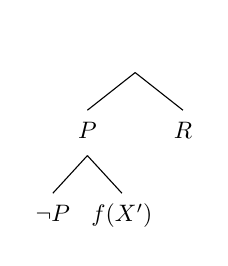
\begin{tikzpicture}
                    \tikzset{execute at begin node=\strut}
                    \tikzset{every tree node/.style={anchor=center, scale=0.86}}
                    \Tree
                    [.{}
                        [.$P$ 
                            [.{$\neg{P}$} ]
                            [.{$f(X')$} ]
                        ]
                        [.$R$ ]
                    ]
                    \end{tikzpicture}
                }
                \only<3>{
                    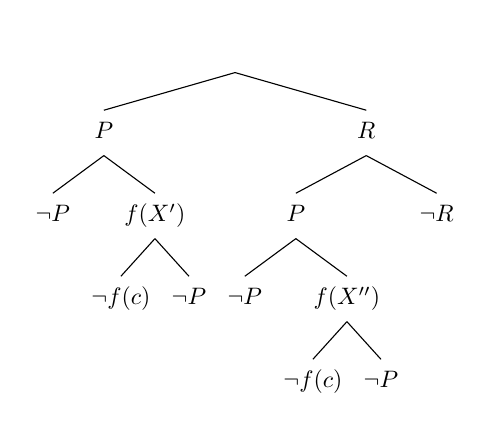
\begin{tikzpicture}
                    \tikzset{every tree node/.style={anchor=center, scale=0.86}}
                    \tikzset{execute at begin node=\strut}
                    \Tree
                    [.{}
                        [.$P$ 
                            [.{$\neg{P}$} ]
                            [.{$f(X')$}
                                [.$\neg{f(c)}$ ]
                                [.$\neg{P}$ ] ] ]
                        [.$R$
                            [.$P$
                                [.$\neg{P}$ ]
                                [.$f(X'')$
                                    [.$\neg{f(c)}$ ]
                                    [.$\neg{P}$ ] ] ]
                            [.$\neg{R}$ ] ]
                    ]
                    \end{tikzpicture}
                }
    \end{columns}
\end{frame}
% \subsection{Semantics of Connection Tableau}

% \subsection{Searching for a Closed Tableau}

\section{Advising with RL}

\subsection{What do we advise?}

\subsection{How do we advise?}

\subsection{Was it worth it?}

\section{Summary}

% TODO DELETE BELOW
\begin{frame}
\frametitle{Paragraphs of Text}
\end{frame}

%------------------------------------------------


\begin{frame}
\frametitle{Blocks of Highlighted Text}
\begin{block}{Block 1}
Lorem ipsum dolor sit amet, consectetur adipiscing elit. Integer lectus nisl, ultricies in feugiat rutrum, porttitor sit amet augue. Aliquam ut tortor mauris. Sed volutpat ante purus, quis accumsan dolor.
\end{block}

\begin{block}{Block 2}
Pellentesque sed tellus purus. Class aptent taciti sociosqu ad litora torquent per conubia nostra, per inceptos himenaeos. Vestibulum quis magna at risus dictum tempor eu vitae velit.
\end{block}

\begin{block}{Block 3}
Suspendisse tincidunt sagittis gravida. Curabitur condimentum, enim sed venenatis rutrum, ipsum neque consectetur orci, sed blandit justo nisi ac lacus.
\end{block}
\end{frame}

%------------------------------------------------

\begin{frame}
\frametitle{Multiple Columns}
\begin{columns}[c] % The "c" option specifies centered vertical alignment while the "t" option is used for top vertical alignment

\column{.45\textwidth} % Left column and width
\textbf{Heading}
\begin{enumerate}
\item Statement
\item Explanation
\item Example
\end{enumerate}

\column{.5\textwidth} % Right column and width
Lorem ipsum dolor sit amet, consectetur adipiscing elit. Integer lectus nisl, ultricies in feugiat rutrum, porttitor sit amet augue. Aliquam ut tortor mauris. Sed volutpat ante purus, quis accumsan dolor.

\end{columns}
\end{frame}

%------------------------------------------------
\section{Second Section}
%------------------------------------------------

\begin{frame}
\frametitle{Table}

\begin{table}
\begin{tabular}{l l l}
\toprule
\textbf{Treatments} & \textbf{Response 1} & \textbf{Response 2}\\
\midrule
Treatment 1 & 0.0003262 & 0.562 \\
Treatment 2 & 0.0015681 & 0.910 \\
Treatment 3 & 0.0009271 & 0.296 \\
\bottomrule
\end{tabular}
\caption{Table caption}
\end{table}

\end{frame}

%------------------------------------------------

\begin{frame}
\frametitle{Theorem}
\begin{theorem}[Mass--energy equivalence]
$E = mc^2$
\end{theorem}
\end{frame}

%------------------------------------------------

\begin{frame}[fragile] % Need to use the fragile option when verbatim is used in the slide
\frametitle{Verbatim}
\begin{example}[Theorem Slide Code]
\end{example}
\end{frame}

%------------------------------------------------

\begin{frame}
\frametitle{Figure}
Uncomment the code on this slide to include your own image from the same directory as the template .TeX file.
%\begin{figure}
%\includegraphics[width=0.8\linewidth]{test}
%\end{figure}
\end{frame}

%------------------------------------------------

\begin{frame}[fragile] % Need to use the fragile option when verbatim is used in the slide
\frametitle{Citation}
\cite{MaLARea}
% An example of the \verb|\cite| command to cite within the presentation:\\~

% This statement requires citation \cite{p1}.
\end{frame}

%------------------------------------------------

%------------------------------------------------

\begin{frame}{Bibliography}
\bibliographystyle{apalike}
\bibliography{../refs.bib}
\end{frame}

%----------------------------------------------------------------------------------------

\end{document} 
